\documentclass[a4paper,10pt]{article}

\usepackage{geometry}
%\geometry{a4paper,left=2.5cm,right=2cm,top=3cm,bottom=2cm}

\usepackage[utf8x]{inputenc}
\usepackage[bookmarks,colorlinks=false,pdfborder={0 0 0}]{hyperref}
\hypersetup{pdftitle={2. Praktikum: Modellierung von Informationssystemen}}
\usepackage{url}
\usepackage[ngerman]{babel}
\usepackage{graphicx}

\parindent 0pt 
\parskip 10pt

\title{2. Praktikum: Modellierung von Informationssystemen}
\author{Andreas Krohn \and Benjamin Vetter}

\begin{document}

\maketitle

\tableofcontents

\section{Zielsetzung und nicht-funktionale Anforderungen}

\begin{description}
  \item[Flexibilität] Das System muss flexibel erweiterbar bzw. adaptierbar sein, damit es bei starken Veränderungen in der Zukunft zügig und kosteneffizient an neue Anforderungen angepasst werden kann.
  \item[Kostensenkung] Das System sollte optimal dabei unterstützen alle Kosten die während der Produktion anfallen zu minimieren.
Insbesondere sollte es Lagerhaltungskosten minimieren und eine minimale Produktionsdauer ermöglichen.
  \item[Zufriedene Kunden] Die Kundenzufriedenheit muss mithilfe des Systems ständig verbessert werden, indem Service schneller geleistet werden kann, Lieferungen schneller die Kunden erreichen und auf besondere Wünsche zügig reagiert werden kann.
  \item[Verbesserte Qualität] Die Produktionsqualität soll durch das System verbessert werden, was ebenfalls die Kundenzufriedenheit erhöht und Folgekosten reduziert.
  \item[Fehlervermeidung] Das System soll Fehlern vorbeugen, indem es Entscheidungen optimal unterstützt.
  \item[Verbesserungsprozess] Das Kaizen-Prinzip, das auf ständige Verbesserung abzielt muss auch Prinzip des Toyota-Produktionssystems sein.
%  \item[Informationstransparenz] 
  \item[Prozess-Standardisierung] Die Prozesse sollen, soweit möglich, mithilfe des Systems standardisiert werden, um die Kompatibilität mit externen Systemen zu erhöhen.
  \item[Prozess-Synchronisierung] Die Prozesse sollen mithilfe des Systems synchronisiert werden, damit es weder zu Engpässen noch zu zeitlichen Verzögerungen kommt.
  \item[Skalierbarkeit] Das System muss mit großen Datenmengen stets performant umgehen können.
  \item[Einfache Bedienbarkeit] Für technisch unversierte Benutzer, wie z.B. Händler, muss das System dennoch einfach benutzbar sein. 
Während Beratungsgesprächen und der Konfiguration werden Systemteile Kunden präsentiert und müssen daher ansprechend gestaltet sein.
Komplexität muss vor den Benutzern verborgen werden.
  \item[Sicherheit] Sensitive Informationen wie personenbezogene Daten müssen vertraulich behandelt werden (Vertraulichkeit). 
Systemausfälle sind fatal, sodass Vorsorge zu treffen ist (Verfügbarkeit). 
Unautorisierte Manipulation von Daten muss ausgeschlossen werden (Integrität).
\end{description}

%- Flexibilität
%- Kostensenkung
%  * Kurze Lagerhaltung
%  * Kurze Produktionsdauer
%  * TTM (Geplante Modelle verkaufen)
%- Zufriedene Kunden
%  * Service
%  * Schnelle Lieferung
%  * auf Wünsche reagieren können (Extras...)
%- Verbesserte Qualität
%- Zuverlässigkeit
%- Fehlervermeidung
%- Kontinuierlicher Verbesserungsprozess
%  * sich selbst optimierendes System
%  * Kaizen-Prinzip
%- Informationstransparenz
%- Prozess-Standardizierung
%- Synchronisierung der Prozesse
%- Skalierbarkeit
%  - muss mit großen Datenmengen performant umgehen können
%- Einfache Bedienbarkeit, für Nicht-Informatiker geeignet
%- Sicherheit (Verfügbarkeit, Vertraulichkeit, Integrität)
%

\section{Problembeschreibung}

Toyota ist ein global agierendes Unternehmen, indem unterschiedlichste Menschen auf unterschiedlichste Weise miteinander mithilfe des Systems kooperieren und kommunizieren müssen.
Unterschiedliche nationale Regulatorien bzw. Gesetze müssen berücksichtigt werden.
Der Produktionsprozess besteht aus vielen Teilschritten die synchronisiert werden müssen.
Toyota hat eine breite Produktpalette unterschiedlicher Modelle und Produktvarianten, was die Komplexität erhöht aber die Bedienbarkeit auch bei geringem teschnischen Know-How nicht negativ beeinflussen darf.
Die Gefahr von Fehlern, die hohe Kosten und negative Außenwirkung nach sich ziehen können, ist aufgrund der hohen Komplexität des Produktionsprozesses sehr groß.
Insbesondere ist die Komplexität der logistischen Prozesse zu nennen, die den Transport zum Kunden, Rohstoffbeschaffung, Just-In-Time Produktion uvm. beinhaltet.
Das System hat mit dem Widerspruch zu kämpfen, dass Standadisierte Bauteile und Prozesse geschaffen und eingesetzt werden sollen, aber variable, individuelle Produkte geschaffen werden.

%- Viele unabhängige beteiligte Instanzen und Personen
%- Synchronizierung der Prozesse
%- Viele Gefahren für hohe Kosten/hohen Imageverlust durch kleine Fehler
%- Toyota operiert auf globaler Ebene ; Multinationalität
%  * Unterschiedliche Regularien zu berücksichtigen (Gesetze, Normen,...)
%- Viele Produkte und Produktvarianten
%- Hohe Komplexität bei möglichst leichter Bedienbarkeit
%- Logistische Probleme
%  * Transport zum Kunden
%  * Rohstoffbeschaffung
%  * Just-in-time Produktion
%- Widerspruch: Standardisierte Bauteile vs. Variable Produkte

\section{UML-Modellierung}

Dieser Abschnitt beinhaltet die von uns angefertigten UML-Diagramme bzgl. der Modellierung des Toyota Production System.

\subsection{fachliches Klassendiagramm}

\begin{figure}[htb]
 \begin{center}
   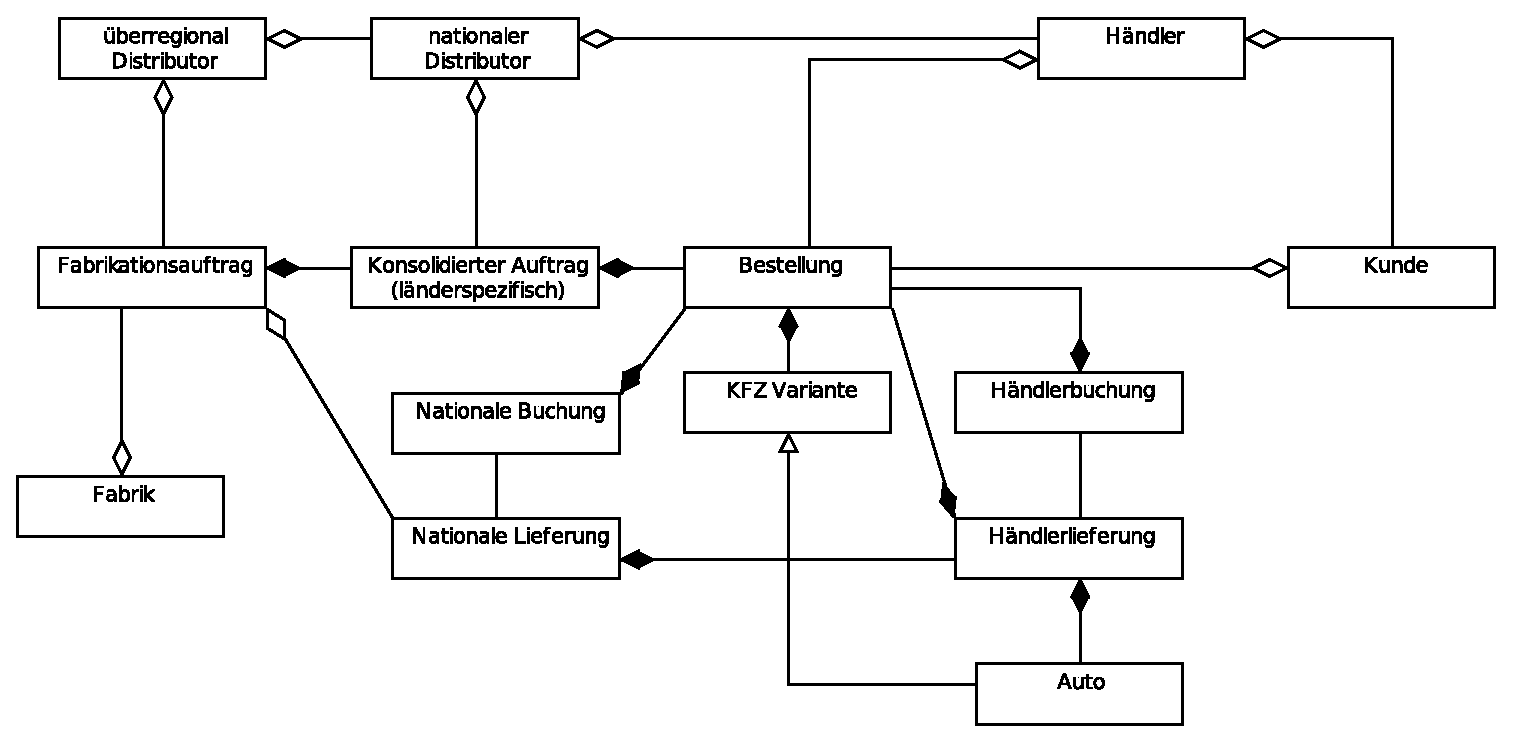
\includegraphics[width=1\textwidth]{fachlichesKlassendiagramm.eps}
    \caption{fachliches Klassendiagramm}
    \label{klassendiagramm}
  \end{center}
\end{figure}

Abbildung \ref{klassendiagramm} zeigt unser fachliches Klassendiagramm.

\subsection{Aktivitätsdiagramme}

\begin{figure}[htb]
 \begin{center}
   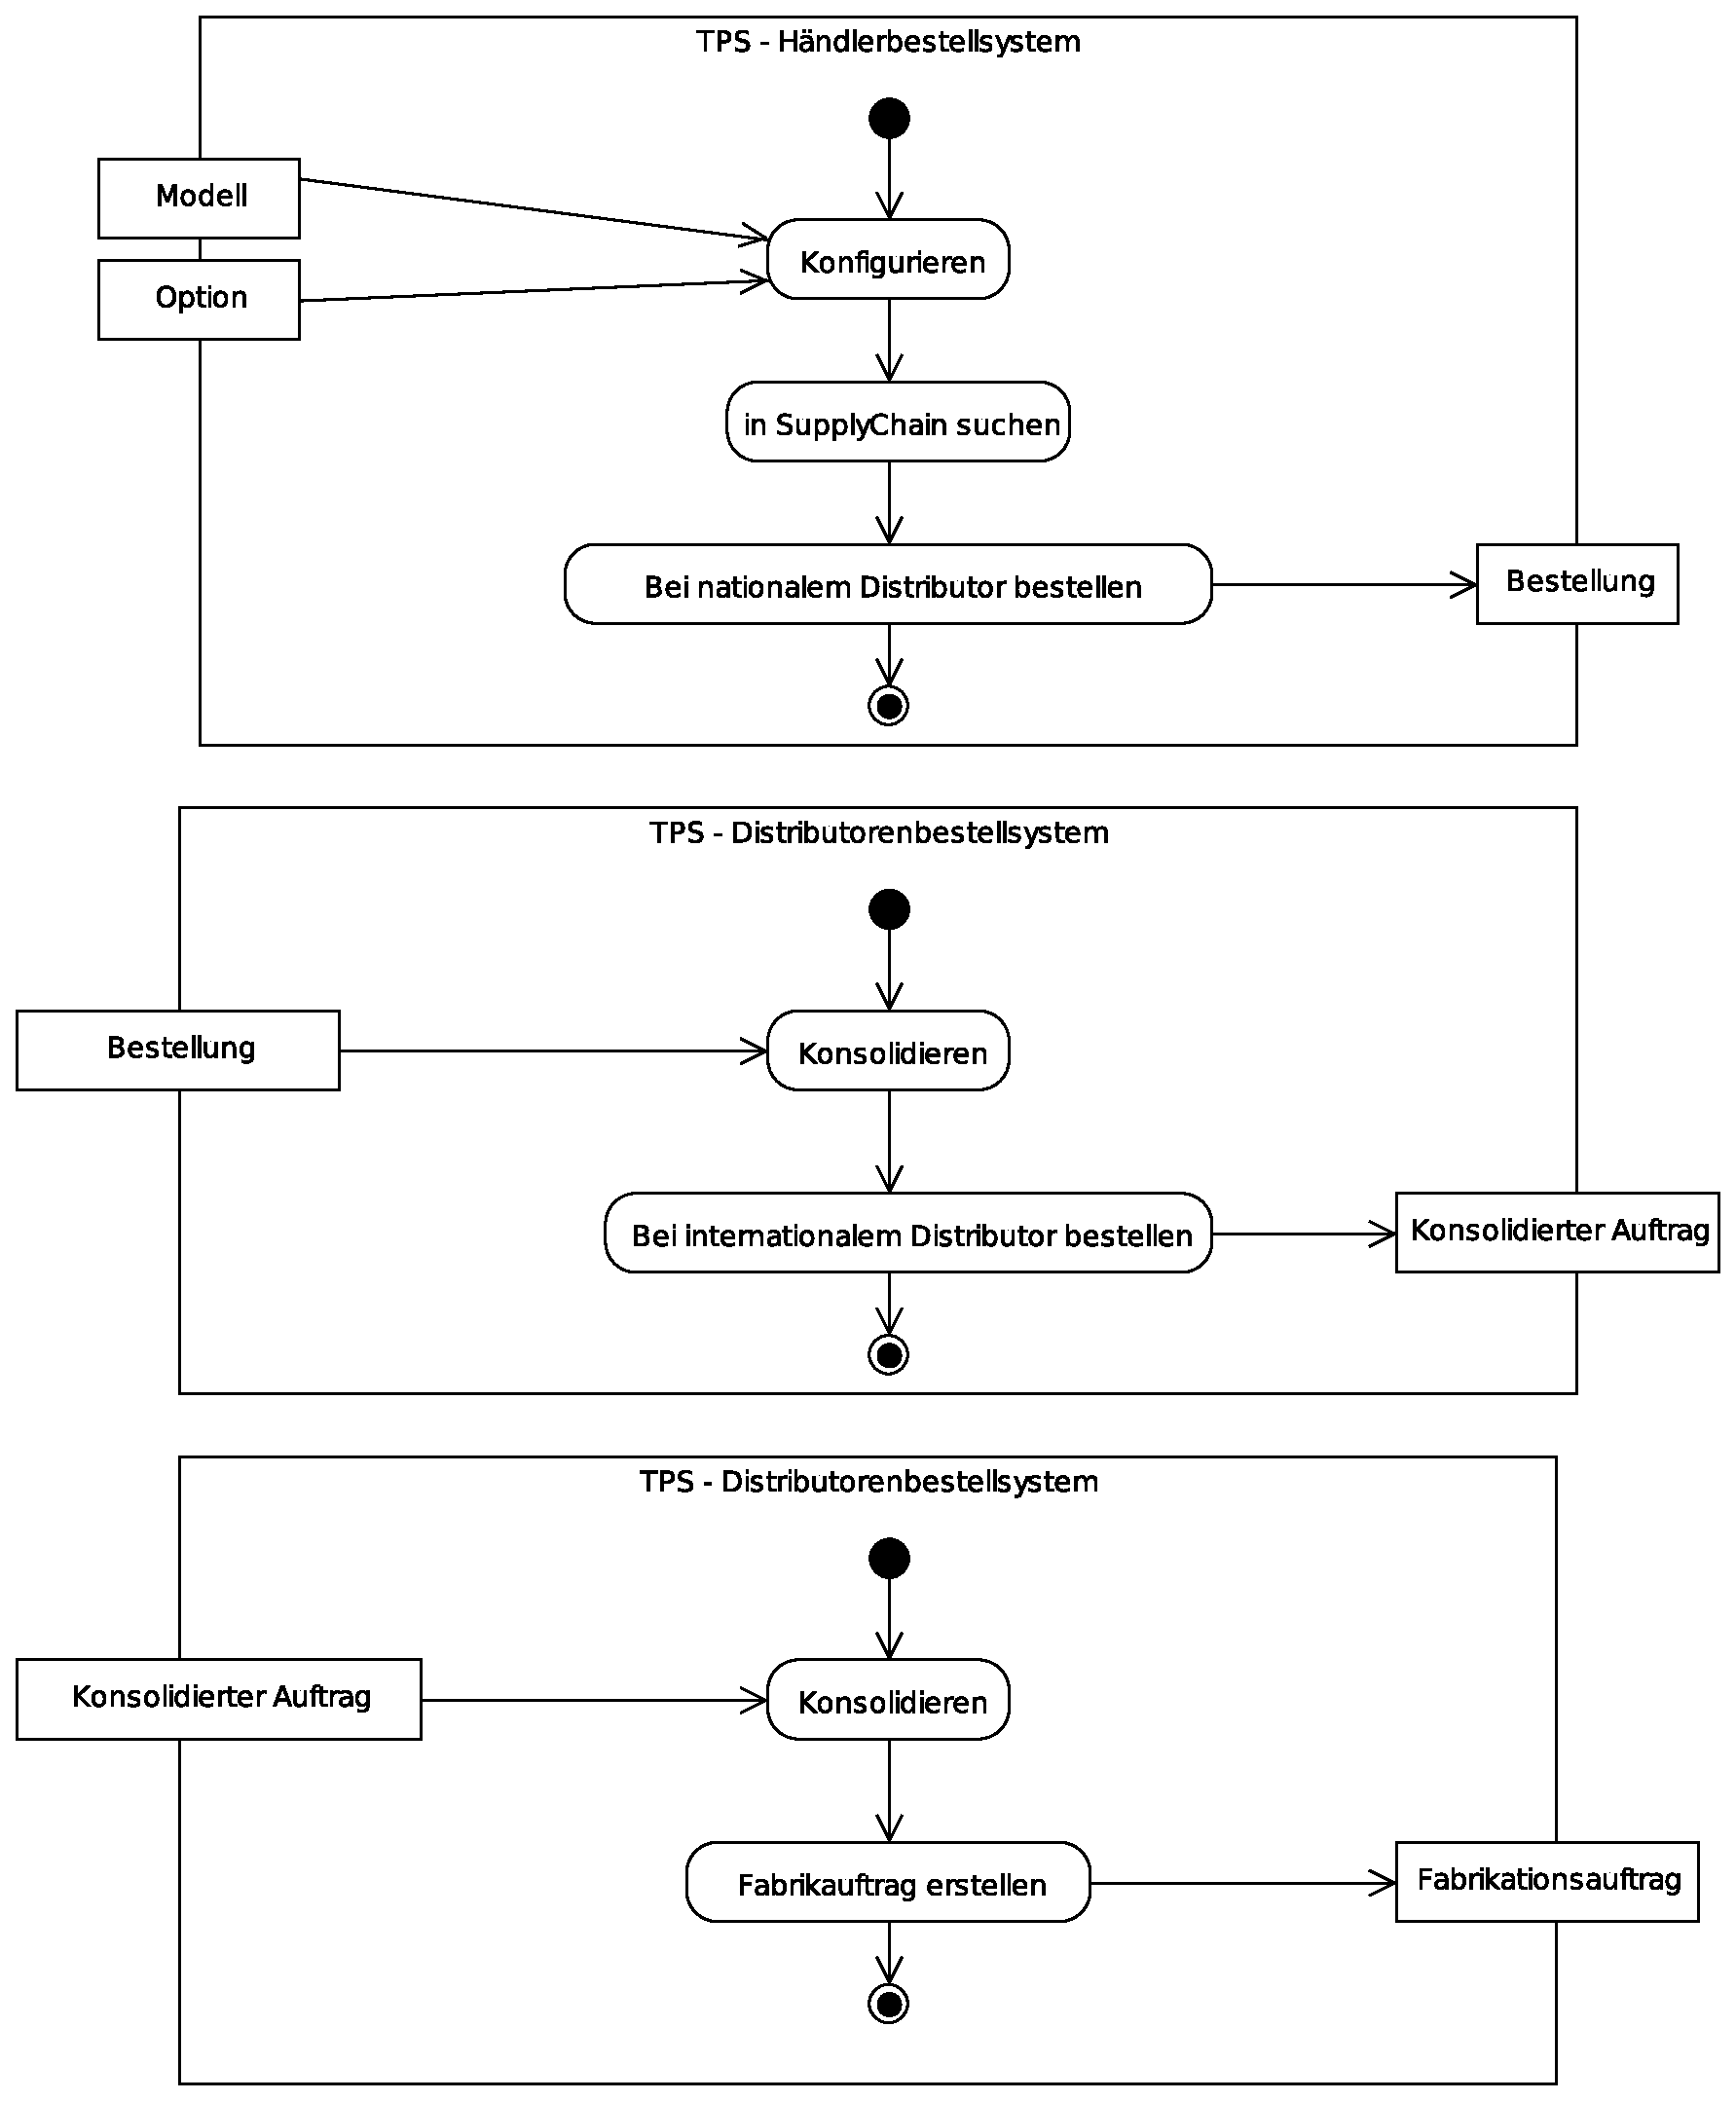
\includegraphics[width=1\textwidth]{activity.eps}
    \caption{Aktivitätsdiagramme 1}
    \label{aktivitaetsdiagramme}
  \end{center}
\end{figure}

\begin{figure}[htb]
 \begin{center}
   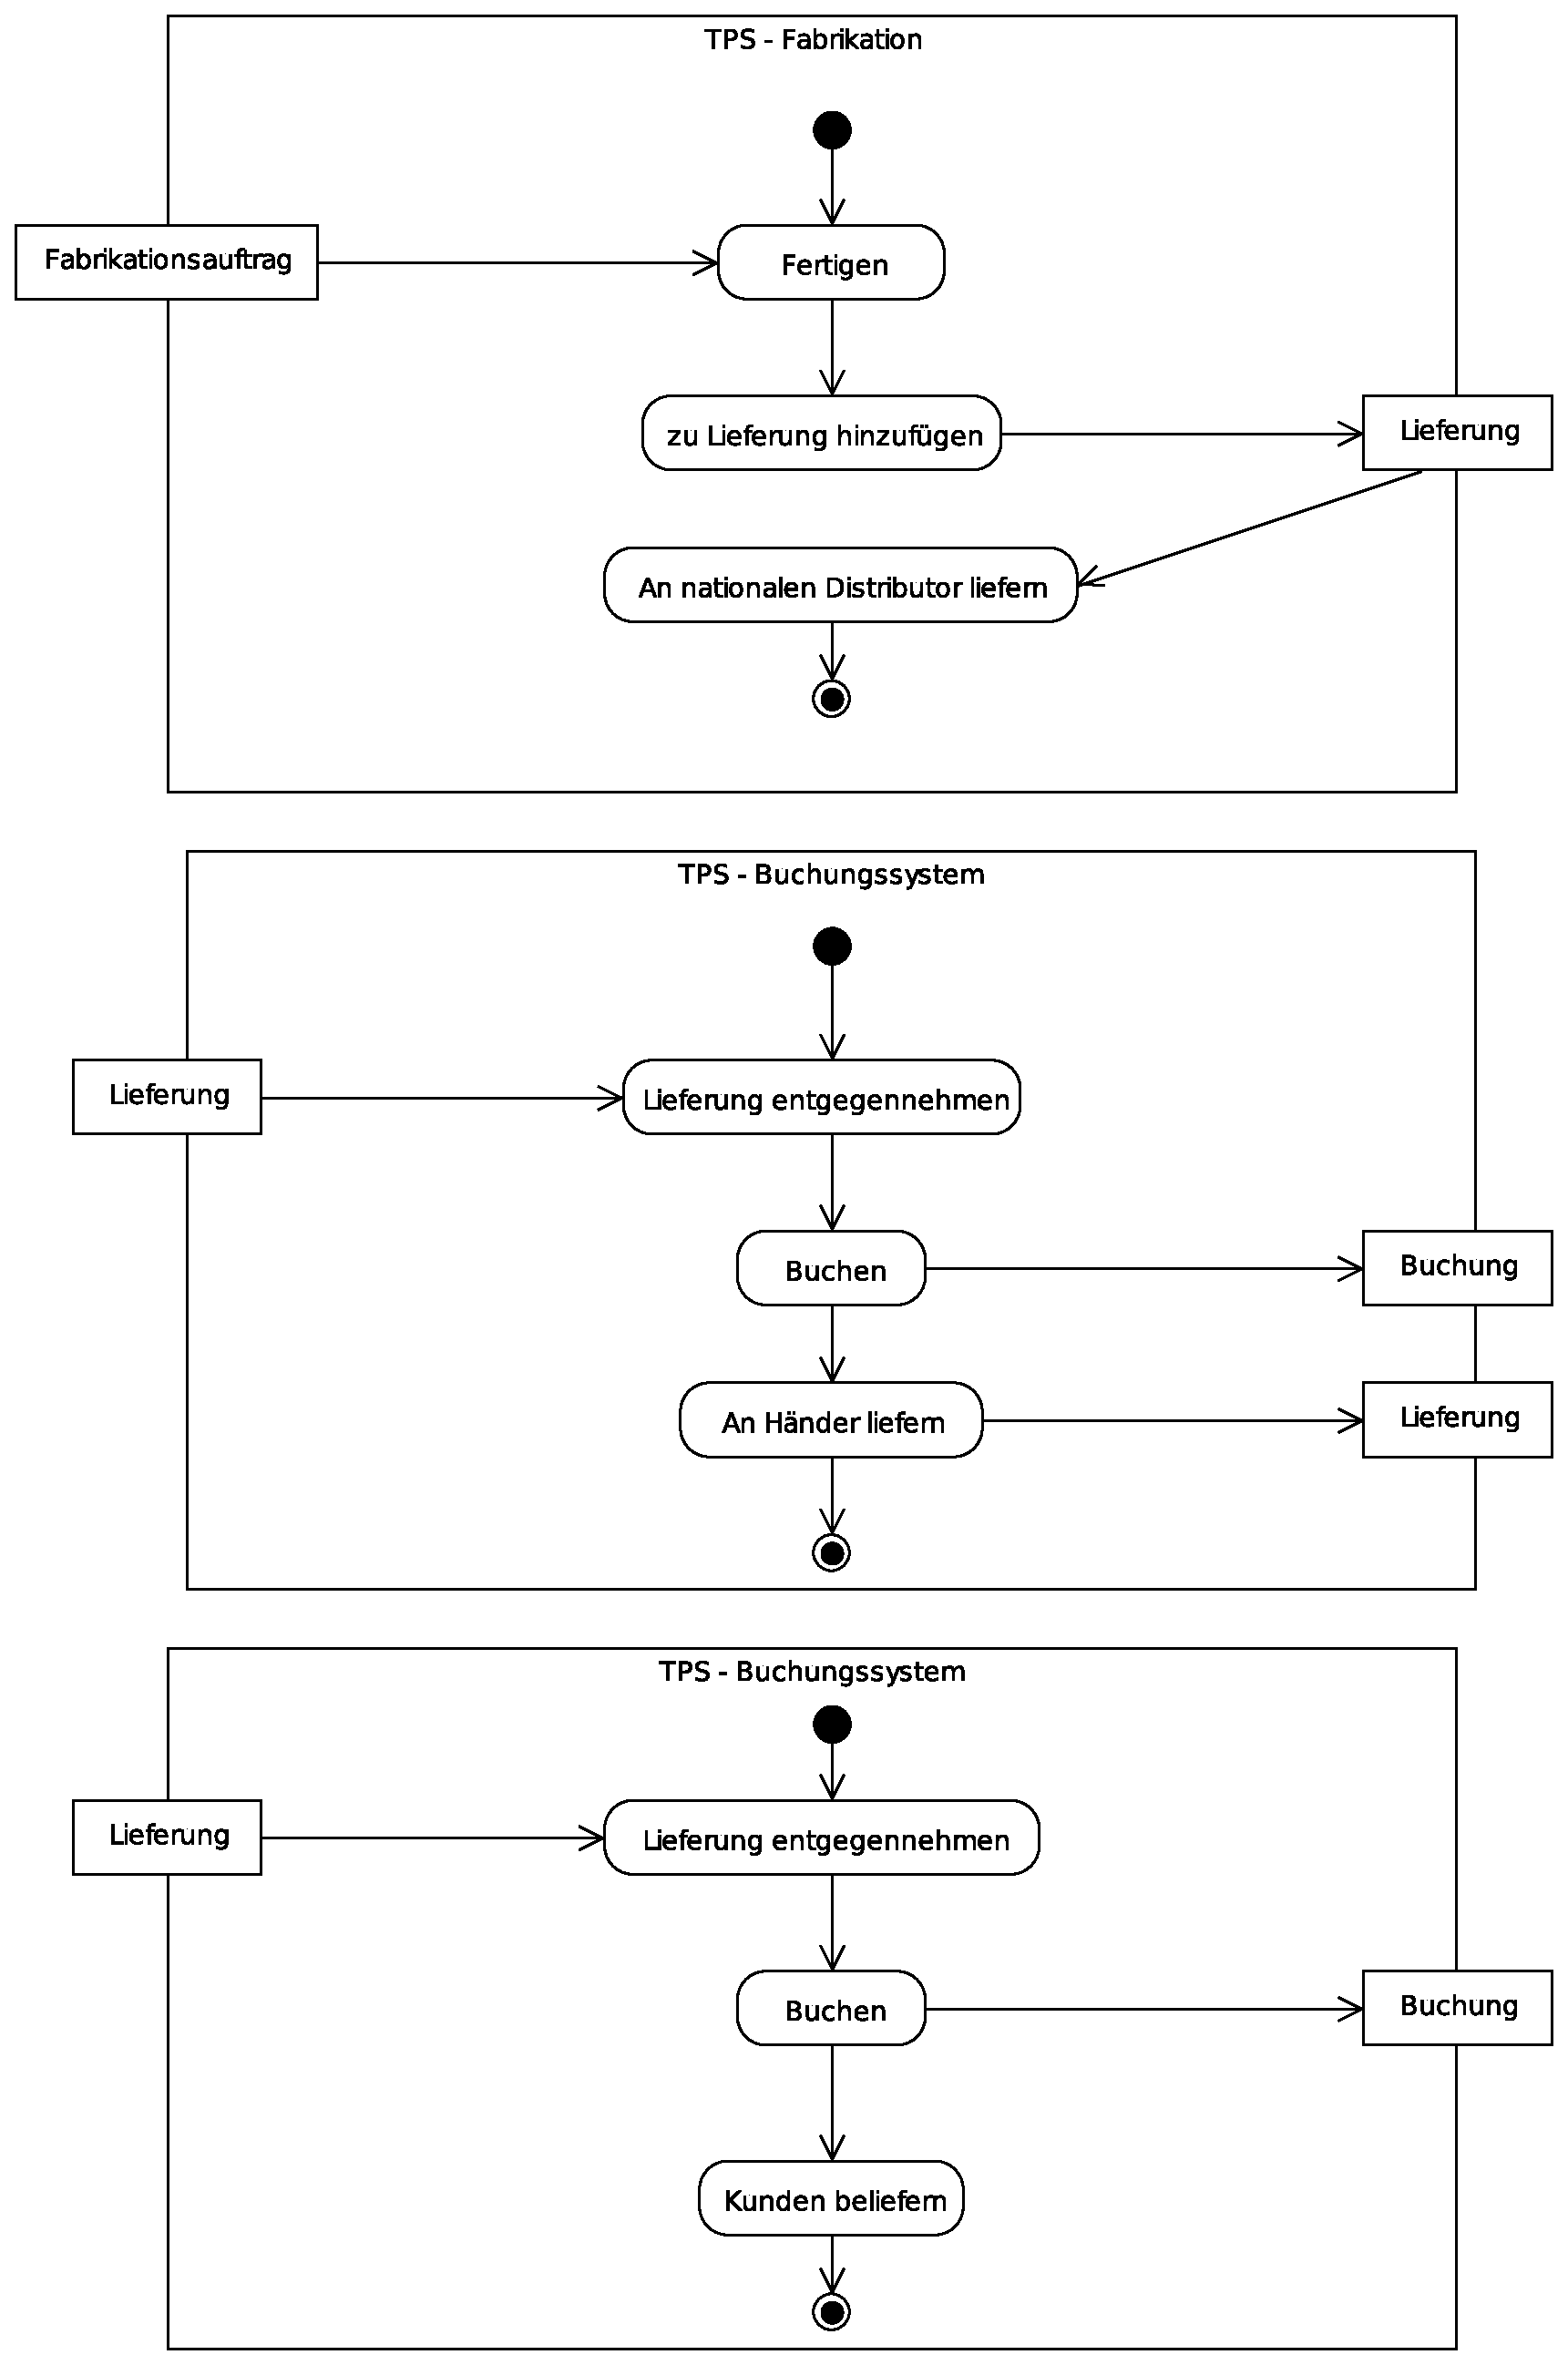
\includegraphics[width=1\textwidth]{activity2.eps}
    \caption{Aktivitätsdiagramme 2}
    \label{aktivitaetsdiagramme2}
  \end{center}
\end{figure}

Abbildung \ref{aktivitaetsdiagramme} und \ref{aktivitaetsdiagramme2} zeigt unsere Aktivitätsdiagramme.

\subsection{Anwendungsfalldiagramme}

\begin{figure}[htb]
 \begin{center}
   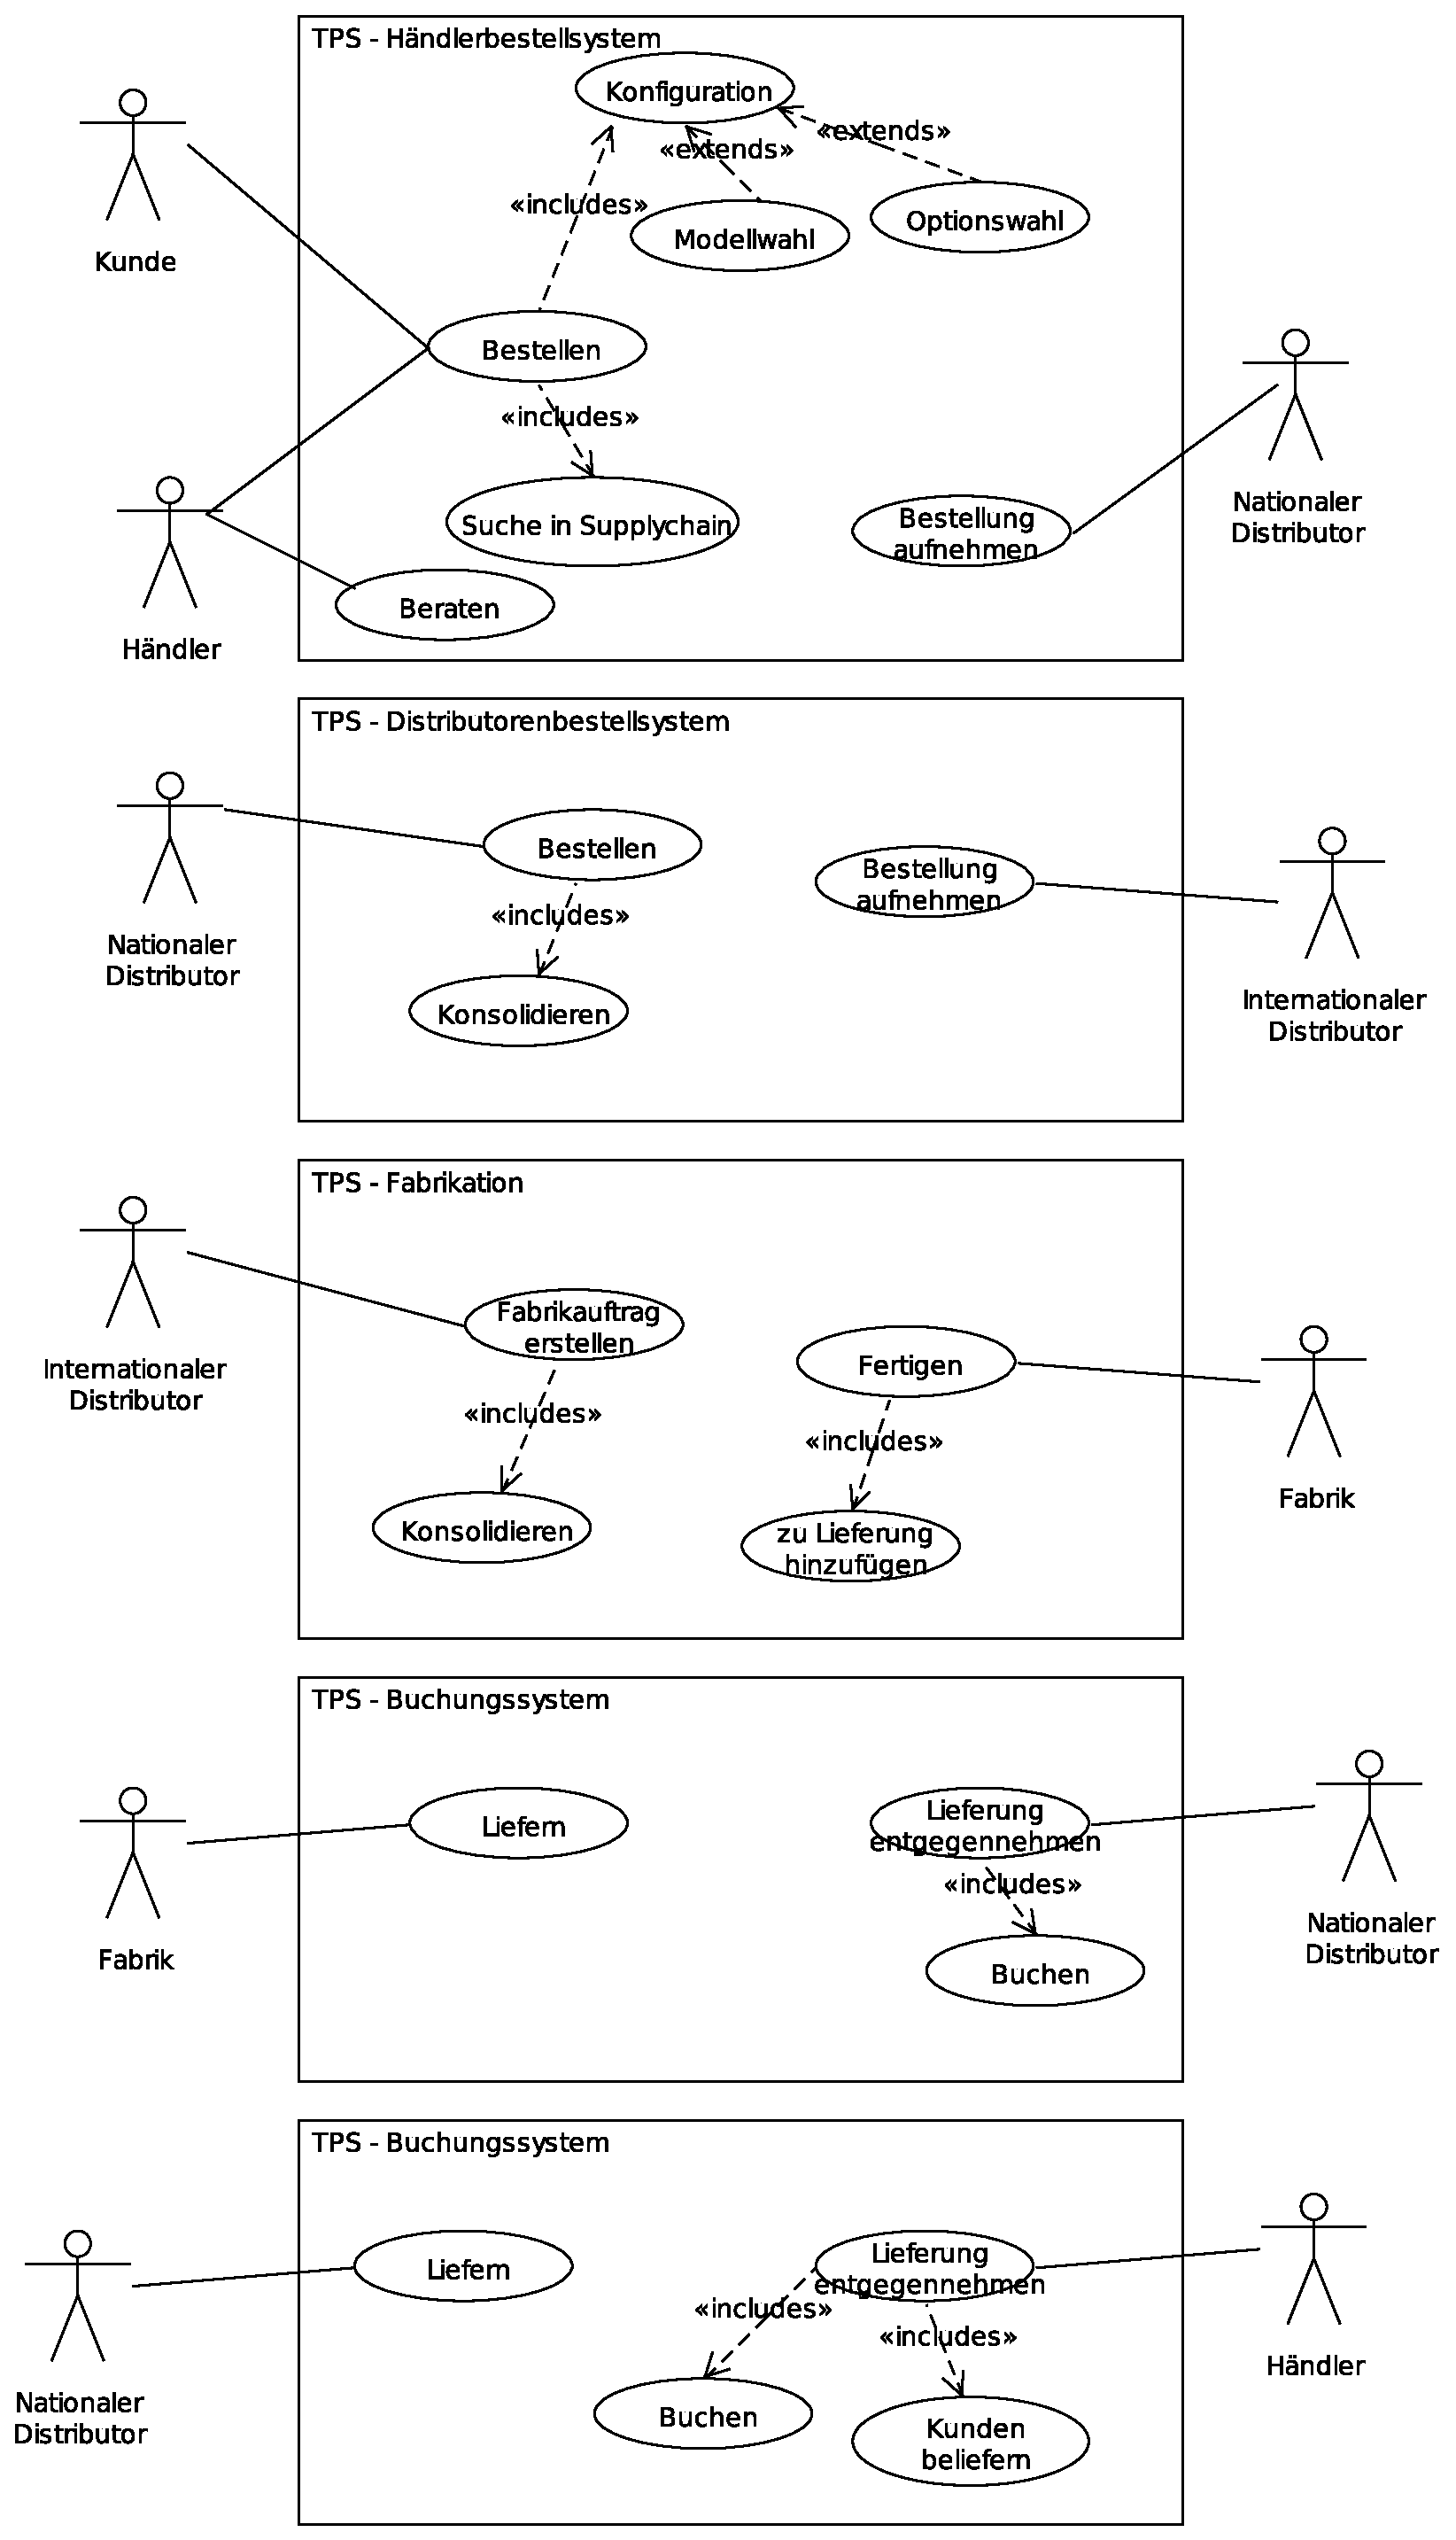
\includegraphics[width=0.9\textwidth]{usecases.eps}
    \caption{Anwendungsfälle}
    \label{anwendungsfalldiagramme}
  \end{center}
\end{figure}

Abbildung \ref{anwendungsfalldiagramme} zeigt unsere Anwendungsfalldiagramme.

\subsection{Komponentendiagramm}

\begin{figure}[htb]
 \begin{center}
%   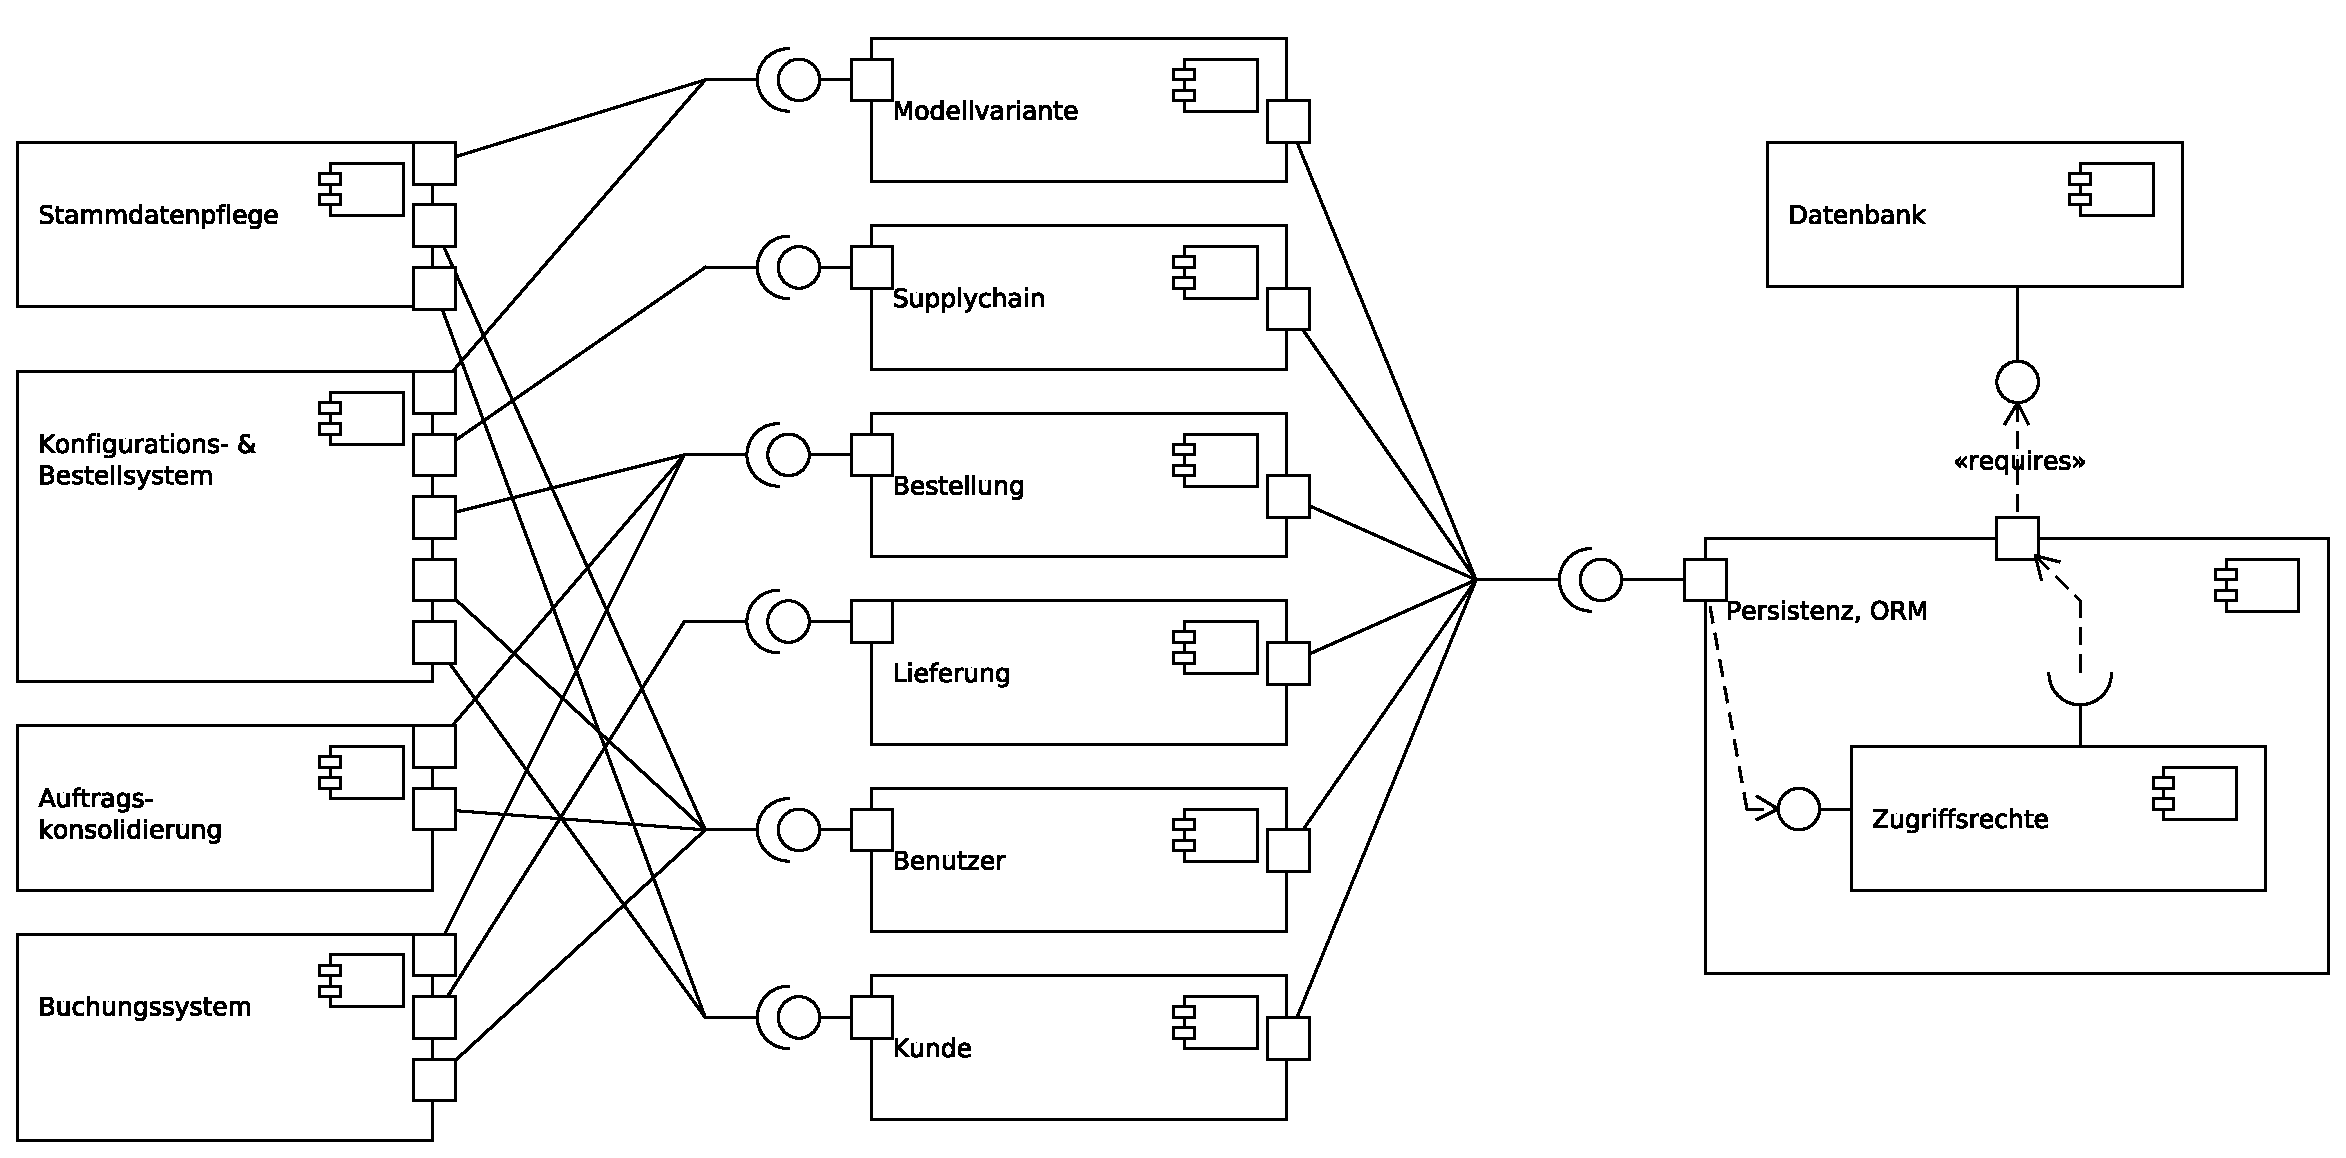
\includegraphics[angle=90,width=0.7\textwidth]{komponentenDiagramm.eps}
   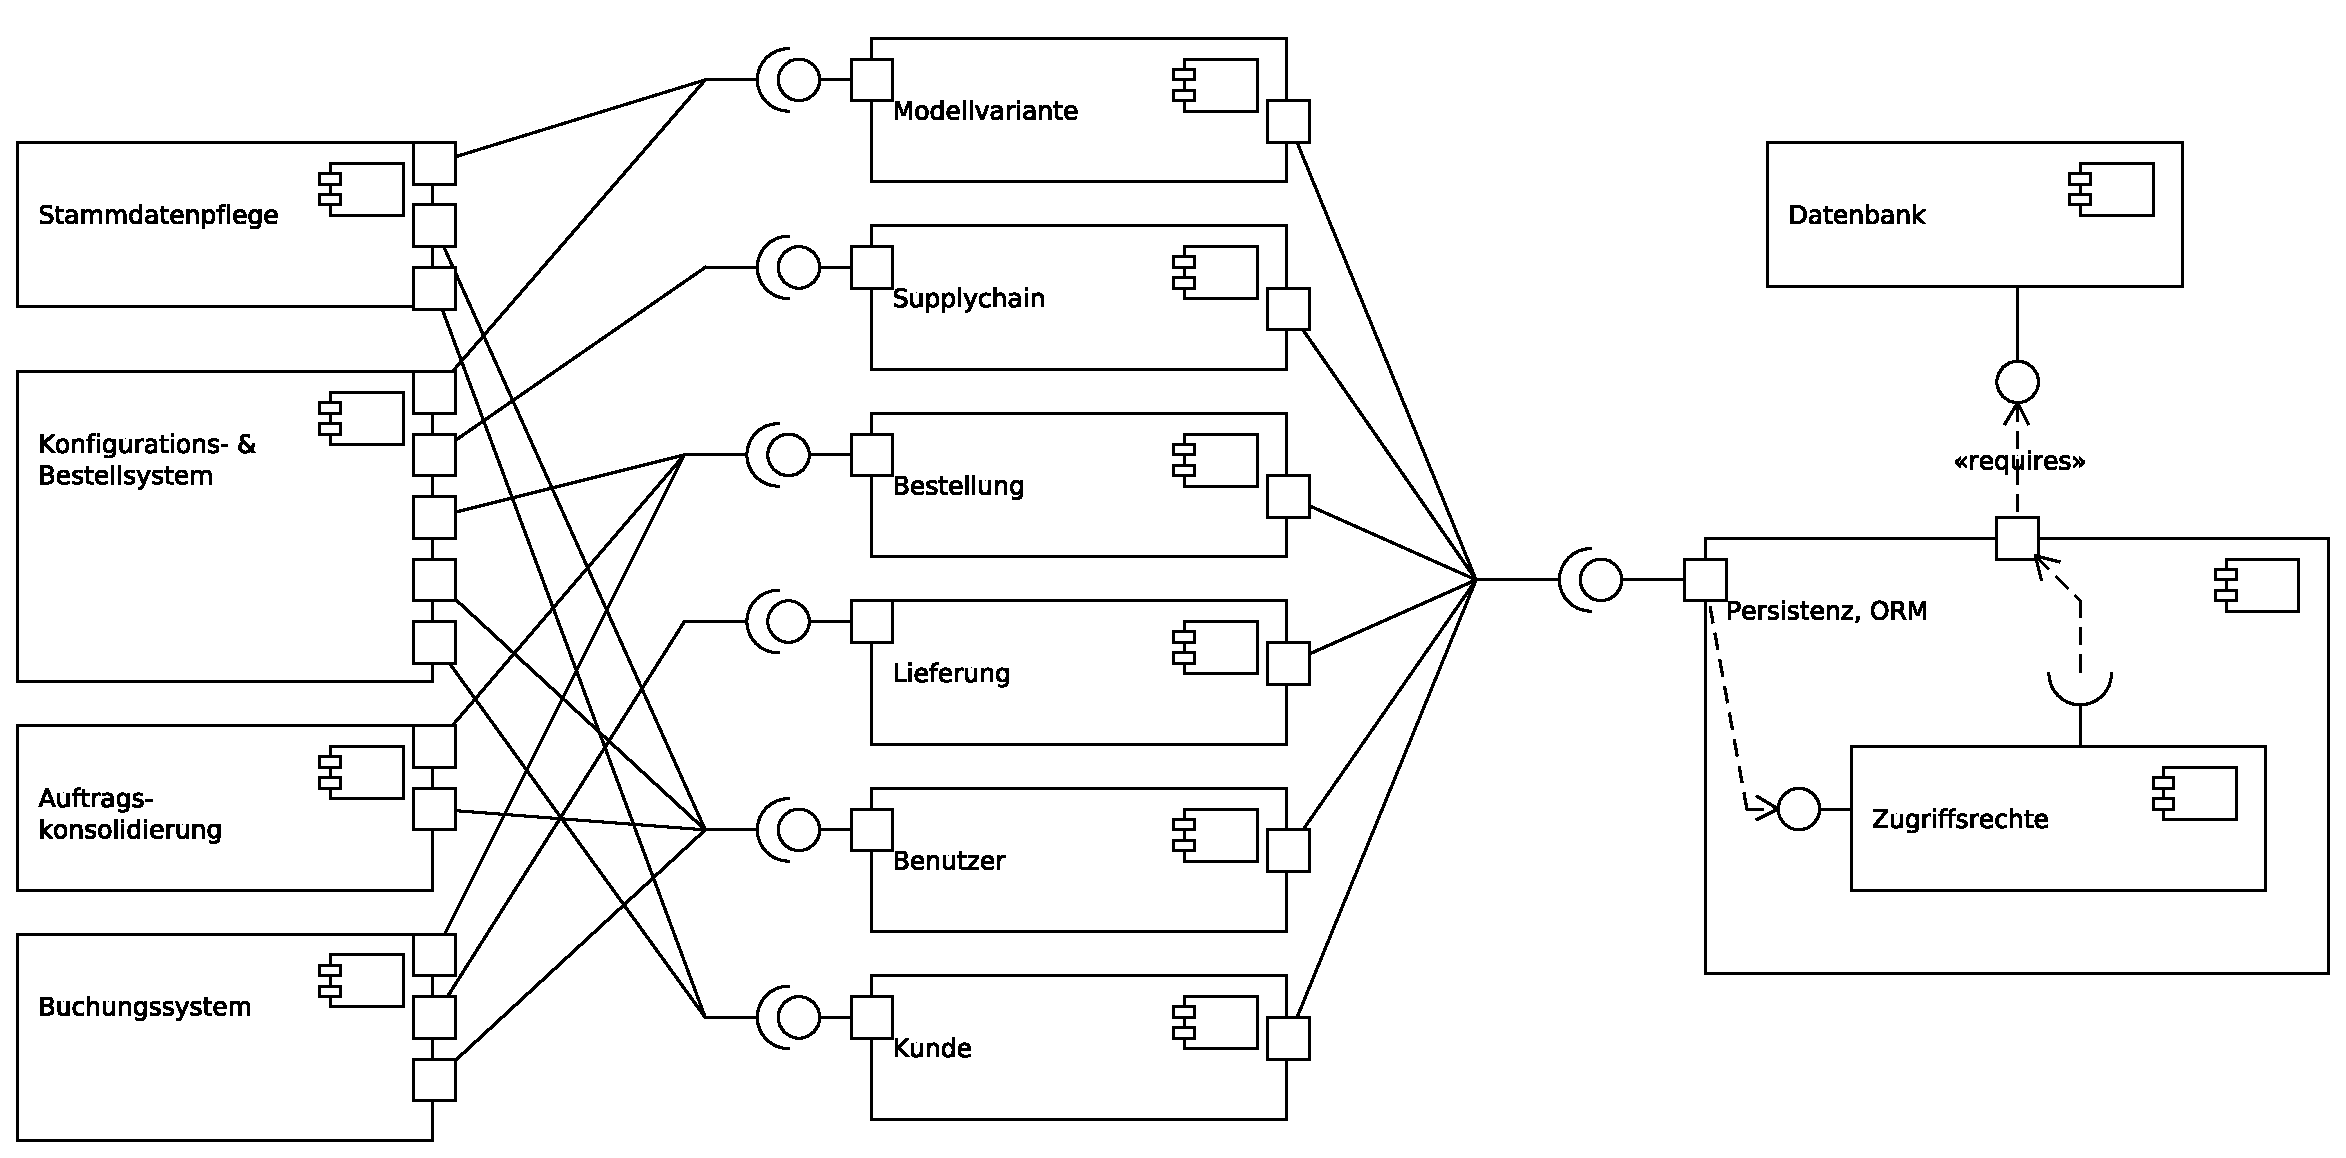
\includegraphics[width=1\textwidth]{komponentenDiagramm.eps}
    \caption{Komponentendiagramm}
    \label{komponentendiagramm}
  \end{center}
\end{figure}

Abbildung \ref{komponentendiagramm} zeigt unser Komponentendiagramm.


\subsection{Dialoge}

Da der Händler die Konfiguration gemeinsam mit dem Kunden vornimmt, muss das Konfigurationssystem anssprechend gestaltet und einfach zu bedienen sein.
Konkret stellen wir uns das Konfigurationssystem wie in Abbildung \ref{konfigurator} vor.

\begin{figure}[htb]
 \begin{center}
\hspace*{-7cm}
   \includegraphics[width=1\textwidth]{dialog_config.eps}
    \caption{Konfigurationssystem}
    \label{konfigurator}
  \end{center}
\end{figure}

Die Benutzerschnittstelle für internationale und nationale Distributoren zur Konsolidierung der Auträge soll übersichtlich, funktional und auf die wesentlichen Aufgaben fokussiert sein.
Eine Skizze, wie diese Benutzerschnittstelle aussehen könnte findet sich in Abbildung \ref{konsolidator}.

\begin{figure}[htb]
 \begin{center}
   \includegraphics[width=1\textwidth]{dialog_konsolidierung.eps}
    \caption{Konsolidierungsdialog}
    \label{konsolidator}
  \end{center}
\end{figure}


\section{Glossar}

\begin{description}
  \item[TPS] Das Toyota Production System ist der Oberbegriff für das gesamte Produktionssystem von Toyota.
  \item[Supply Chain] In der Supply Chain (englisch Liefer- oder Versorgungskette) können Händler zusammen mit Kunden nach bereits gefertigten Autos suchen, die der gewünschten Konfiguration möglichst stark entsprechen.
  \item[Händler] Ein Händler ist der direkte Bezugspunkt für Endkunden.
  \item[Nationaler Distributor] Ein nationaler Distributor nimmt Händlerbestellungen entgegen, konsolidiert Händlerbestellungen und gibt Bestellungen bei internationalen Distributoren auf.
  \item[Internationaler Distributor] Ein internationaler Distributor nimmt Bestellungen nationaler Distributoren entgegen, konsolidiert die Bestellungen und gibt Farbikbestellungen auf.
  \item[Fabrik] Eine Fabrik ist zuständig für die Fertigung von Fabrikaufträgen und leitet die Lieferungsprozess ein.
  \item[Kaizen-Prinzip] japanisch "`Verbesserung zum Besseren"' bezeichnet eine japanische Lebens- und Arbeitsphilosophie. Im Zentrum des Kaizen-Prinzips steht das Streben nach ständiger Verbesserung.
\end{description}

\end{document}

